\documentclass[11pt,oneside,a4paper]{article}
\usepackage[utf8]{inputenc}
\usepackage{textcomp}
\usepackage{setspace}
\usepackage{graphicx}
\title{Design Document \\ for \\ Multi-user Infinite Canvas Thingy (MICT)}
\author{Don Huckle, Ben Kaplan, Mark Wyrzykowski, Rob Wiesler}
\begin{document}
\maketitle
\tableofcontents
\pagebreak

\section{Tools}
  The Tools are the heavy lifters of the program. Each Tool is self-contained
  and is responsible for drawing itself on at least three kinds of graphics
  contexts:
 \begin{itemize}
  \item The context of the user's viewport
  \item The context of the infinite canvas, as it exists on the server
  \item The context of the viewports of other users who are viewing a particular section of canvas
 \end{itemize}

 \subsection{Serializing the Tools}
  Each of the Tools will be stored on the server and transmitted to the Client
  upon log-in. To facilitate this, each of the Tools should be implemented in
  Jython. Preliminary research shows that the Jython classes can be serialized
  using Java's ObjectOutputStream, but this has not yet confirmed satisfactorily.

 \subsection{Mouse Events}
  The Tool is expected to implement MousePressed, MouseDragged, and
  MouseReleased methods that are called when the mouse is pressed, moved (while
  pressed), and then released while this Tool is active. Each of these methods
  returns a String, which will be transmitted to the server in order to apply the
  change to the global canvas.  These methods are passed the canvas's Graphics
  object and the Point on the canvas where the event was fired from.

 \subsection{Drawing to a Graphics Context}
  Here, the Tool will be passed a String generated by the tool and a Graphics
  object to draw the figure on. The changes to the canvas generated by this
  method should be identical to the changes generated by the tool on the client
  side. To this end, Tools acting on a user's local viewport will only draw to
  the local graphics context based on the same String passed to the server-side
  Tool incarnation.

 \subsection{Tool Properties}
  Each tool will need to know its name in both human-readable and shortened
  internal forms, and an icon. The icon and human-readable name (presented as a
  tooltip) will be used on the client-side to represent the tool to the user.

\section{Client Program Specification}
 This section describes the layout of the client program. It will discuss all
 the components of that program and how they interact with each other. There
 are five main parts to client-side architecture:
 \begin{itemize}
  \item the Client
  \item the ClientState
  \item the Toolbox
  \item the Canvas Control Panel
  \item the Canvas Viewport
 \end{itemize}

 \subsection{Client}
  The root of the client program is the Client class. This is the
  application/applet itself. Other than initializing the other components and
  coordinating communication between them, it is also responsible for setting the
  location of the canvas, either as a result of initially connecting to the
  server, through a jump command, or by panning the viewport. The Client will
  hold a ClientState object that stores the shared settings. In addition, the GUI
  will consist of three components:
  \begin{itemize}
   \item the Toolbox
   \item the Canvas Control Panel
   \item the Canvas Viewport
  \end{itemize}

 \subsection{ClientState}
  A single ClientState object will be initialized for each instance of the
  program. The ClientState object will be used to store the shared state. Any
  field that needs to be accessed and modifed by multiple classes should be
  placed in here, including but not limited to the currently selected tool and
  color, the current location of the canvas, and the persistent connection to the
  server. The use of a singleton structure for shared state will reduce the
  coupling between all the components, slightly increasing complexity, but
  opening up the client-side architecture for potential future improvements, such
  as multiple viewports and simultaneous connections to multiple servers.

 \subsection{Toolbox}
  The Toolbox will contain a series of Tools. Each Tool (which extends the
  abstract class mict.tools.Tool) shall be defined in Jython so that we can
  serialize the class and transmit it from the server to the client. This way,
  every client will support every tool the server has without any prior
  configuration on the part of the user. Additionally, this provides us with an
  opportunity to leverage a more consistent Tool architecture than might exist
  should both a client- and server-side implementation exist for each Tool.
  \subsubsection{ToolButtons}
   For each Tool, the Client will make a ToolButton. ToolButton is a subclass
   of JButton.  It has an ActionListener that sets the associated tool as the
   active tool within ClientState when the button is pressed. Each ToolButton will
   set its icon and tooltip as directed with the underlying Tool class.

 \subsection{Canvas Viewport}
  The Canvas Viewport is a JPanel embedded in the Client UI that will display a
  section of the overall canvas. The user will draw on the Viewport with a Tool
  in order to modify the canvas, and other users modifications will be updated
  here.\\\\
  The Canvas shall have a single MouseListener, which will wait for
  MousePressed, MouseDragged, and MouseReleased events and dispatch those events
  to the currently selected tool. As these methods are called, the Canvas shall
  transmit the serialized commands to the server via the Client Connection, which
  will be discussed later in this document.

 \subsection{Java-Python Bridge}
  There will be a single Java class and a single Python module
  (\verb JythonBridge.java  and \verb javabridge.py ) to facilitate communication
  between Jython and Java components. Any Java component that needs to access
  something from Jython should go through JythonBridge. Because of the way Jython
  works, Python components can access the Java libraries directly if they need to
  extend them (for instance, extending Tools). However, if they require an
  instance of a Java object, they should go through javabridge.

 \subsection{Canvas Control Panel}
  Apart from normal editing actions, users with elevated privileges will have
  access to a separate tab in the Toolbox. In this tab there will be additional
  functions available based on the level of the user. Among these functions are
  the ability to lock parts of the canvas, kick users, move other users around
  the canvas, ban/unban users, and modify the permissions of other users.\\\\
  When a user locks an area, they gain power over that area and are the only one
  (Administrators not included) that can edit it unless they decide to invite
  other users to edit the area. The administration panel is context-aware, so
  options present in the Control Panel deactivate when the user leaves the area
  in which he or she has elevated privileges, and re-activate upon return.\\\\
  Administrators have this power over the entire canvas. They can lock and
  unlock sections even if that section had been locked by another user.\\\\
  In addition to modifying privileges for the canvas, Administrators can
  reconfigure the canvas in real time, and can save the canvas and stop the
  server gracefully.
  \begin{itemize}
   \item
    The options in this panel will be implemented as Tools if possible, and
    will only be dealt with as a special case if the Tool interface does not
    provide all of the required functionality of the option.
   \item
    These controls change as the user moves over the canvas. The server will
    communicate to the Client which sections are valid options for the user given
    the user's current location on the canvas. For instance, the server may be
    configured such that a particular user owns reserved areas of the canvas.
    Naturally in this scenario, the administrative controls for reserved segments
    will be contextuallized by the position of the user on the canvas. Therefore,
    in a public area, the administrative controls of a user of a locked area
    somewhere else will be diabled in the Canvas Control Panel, and the network
    protocol will stop responding to administrative actions.
   \item
    Users will only be presented with options appropriate to their
    permissions. If they do not have permission to acquire sections for
    instance, they will not see that button presented to them. If they have
    permission but are unable to acquire it (for instance, if someone else
    owns it), the button will be inactive.
   \item
    Administrator-level users will have available to them in the Control Panel
    options to trigger the Canvas.User.Kick, Canvas.User.Ban, and
    Canvas.User.Pardon functions from section 3.4 of the requirements document.
  \end{itemize}

 \subsection{Launching the MICT Client}
  When the program is launched as an application, the Toolbox will be empty and
  the Canvas Viewport will be replaced by two JTextFields, a JPasswordField, and
  a JButton. The first JTextfield will be used to enter the server to connect to.
  The second will be the username, and the JPasswordField will be used to enter
  the password. The JButton will tell the client to connect to the server
  specified with the given log-in credentials. If login is successful, the fields
  will be replaced with the Canvas Viewport. This implements the Canvas.Connect
  requirement mentioned in section 3.1 of the SRS document.\\\\
  In the case that the client is launched as an applet, the above behavior will
  occur, with the exception that the presence of an HTML applet parameter
  providing the name of the server will result in the absence of a text area used
  to specify the server.
  \begin{itemize}
   \item
    When the user presses the log-in button, the ClientConnection will be
    created. Upon successful connection, the Client will create the ClientState
    object, retrieve the Tools from ther server and create the ToolButtons, and
    then add the Canvas Viewport and set the associated Graphics in the
    ClientState.
   \item
    Depending on the user's permissions and location, the Canvas Control panel
    may also be populated to hold the interface for administrative actions
    specified in Section 3.3 of the Software Requirements Document.
  \end{itemize}

\section{Client-Server Specification}
 The client server interaction is based on a TCP connection between the server and the client.  
 In per-user communication there are three major threads driving interaction:
 \begin{itemize}
  \item the server's Waiter thread
  \item the client's ClientConnection thread
  \item the client's GUI thread
 \end{itemize}

 \subsection{Connecting to the Server}
  Upon clicking the ``connect'' button at the start of the program execution,
  the client GUI thread will generate a ClientConnection object responsible for
  maintaining a persistent connection with the server. On the server side exists
  a corresponding Waiter object that represents the user within the architecture
  of the server. After the initial SSL handshaking, the client will transmit its
  username and a secure hash of its password and the hostname. This is for
  security reasons as follows:
  \begin{itemize}
   \item
    The password must be hashed at least on disk to limit the risk of revealing
    the user's password to persons with hard or soft access to the server.
   \item
    The password must also be hashed before being handed over to the server to
    avoid giving the server administrator a password potentially in use on other
    servers and services.
   \item
    Since a malicious administrator with access to the hashed version of a
    password may potentially modify the client to send a hashed password to another
    server, thus gaining admission, the password must be hashed along with
    server-specific information in order for the hashed password to maintain
    validity for only a single server.
   \item
    The Internet-facing hostname of the server\footnote{As in
    \texttt{rdebase.case.edu} as opposed to \texttt{rdebase}} is ideally suited for
    this task. For one, if a server-wide arbitrary string were given to the user as
    the server-specific string, it would be simple to momentarily change the
    server-specific string on a malicious server to match the one used on another
    server, rendering the measure useless. However, the relatively constant
    hostname is not so easily spoofed by a malicious administrator, since the
    client is aware of its true value even before connecting\footnote{Except
    notably in the case of Applet-based deployments}.
  \end{itemize}
  If the authentication provided by the client is accepted by the server, the
  server will respond with a Message of the Day (MotD), and an initial set of
  coordinates. The client should respond with an optional request to change
  location, and notify the server of the desired width and height of its
  viewport, which the server should respond to with an initial render of the
  canvas at that point, sized to fit the viewport.

 \subsection{Client-Side Generated Communication}
  When an event is triggered on the client side, it will often result in a
  message being sent to the ClientConnection object. This object will then
  package the information in a protocol wrapper, and pass it on to the server. To
  prevent network communications from locking up server- or client-side logic,
  both the ClientConnection and Waiter objects should handle incoming messages in
  a separate thread. Operations that will cause communication to be generated by
  the client include \verb mouse_clicked , \verb mouse_dragged , and \verb mouse_released  events.
  These events have event handlers associated with them that instruct the active
  Tool to encode the user's current actions into a String, which the client then
  packages with the internal name of the Tool and sends to the Waiter object on
  the server side.

 \subsection{Server Response to User Edits}
  When the Waiter object gets an instruction to apply a tool to the canvas, it
  pushes the request, along with the user's name and viewing rectangle,
  down-archecture to the server's CanvasManager object. The purpose of the
  Canvas Manager is to handle the intricacies of the infinite canvas abstraction.
  The Canvas Manager retrieves the tool corresponding to the tool name in the
  message from the ToolManager entity, and locates the Chunk object closest to
  the center of the user's viewport. It then creates a ChunkGraphics graphics
  context for that chunk, which performs three functions:
  \begin{itemize}
   \item
    It handles the translation from the user's viewport coordinate system into
    the coordinate system of the infinite canvas, using offsets provided by the
    Waiter object's bounding rectangle field.
   \item
    It keeps track of drawing operations that extend over the edge of the
    Chunk's boundaries, and applies those draw operations\footnote{with appropriate
    offsets, using another ChunkGraphics context} to the Chunk objects that exist
    beyond the borders of the initial Chunk object.
   \item
    It prevents Tools wielded by a user without permission to write in an area
    from modifying said area, which may or may not have be delimited by Chunk
    boundaries. For instance, if user Bob controls a smallish circular area and
    Alice does not have write permissions within that area, a line drawn by Alice
    through Bob's circular area and extending some distance to either side will
    resolve on the canvas on the outside of Bob's area, but on inside. In response
    to an illegal write attempt, it passes a message back to the client, which
    notifies the user in a subtle way that something went wrong, and eventually
    updates the user with a correct version of the visible canvas.
  \end{itemize}
  If there are other users active in the region of Chunks that were modified
  by the Tool, the Canvas Manager locates them among the list of Waiter objects
  and pushes updates to the affected areas out to them, with care to only update
  the intersection of the affected areas and the views of the other users.

 \subsection{Server storage of Canvas Chunks}
  Since an infinite\footnote{or, at least arbitrarily large} canvas will not
  neccessarily fit into memory all at once, a backend layer that consists of the
  CanvasManger and the DatabaseLayer objects performs some abstraction of the
  canvas into Chunks, as mentioned before, and stores only a limited amount of
  them in memory at once. The maximum number of Chunks in memory is governed by
  the \verb MAXCHUNKS  field of the CanvasManager class. When the Canvas Manager
  gets a request for a Chunk, it servers its cache for the matching Chunk. If it
  finds it, it returns it. Otherwise, it requests the Chunk from the Database
  Layer. If it needs to, it passes inactive Chunks back onto disk by returning
  them to the Database Layer, which saves them to the database.\\\\
  In case of catastrophic system failure, a thread internal to the Canvas Manager
  periodically passes all Chunks back to the Database Layer to save them.

 \subsection{Server-Side Generated Communication}
  When the Server has some action that it needs the client to take, such as
  updating the client's canvas with edits made by another user, the server will
  send an injunction to the client specifying either an update to the client's
  canvas or a message to hand to the user. The client connection Because Java's
  Swing architecture is not thread safe, the client will invoke the operation is
  a roundabout manner via \verb|SwingUtilities.invokeLater(Runnable)|.

\pagebreak
\section{Appendix: UML Depemdency Diagram}
 \begin{center}
  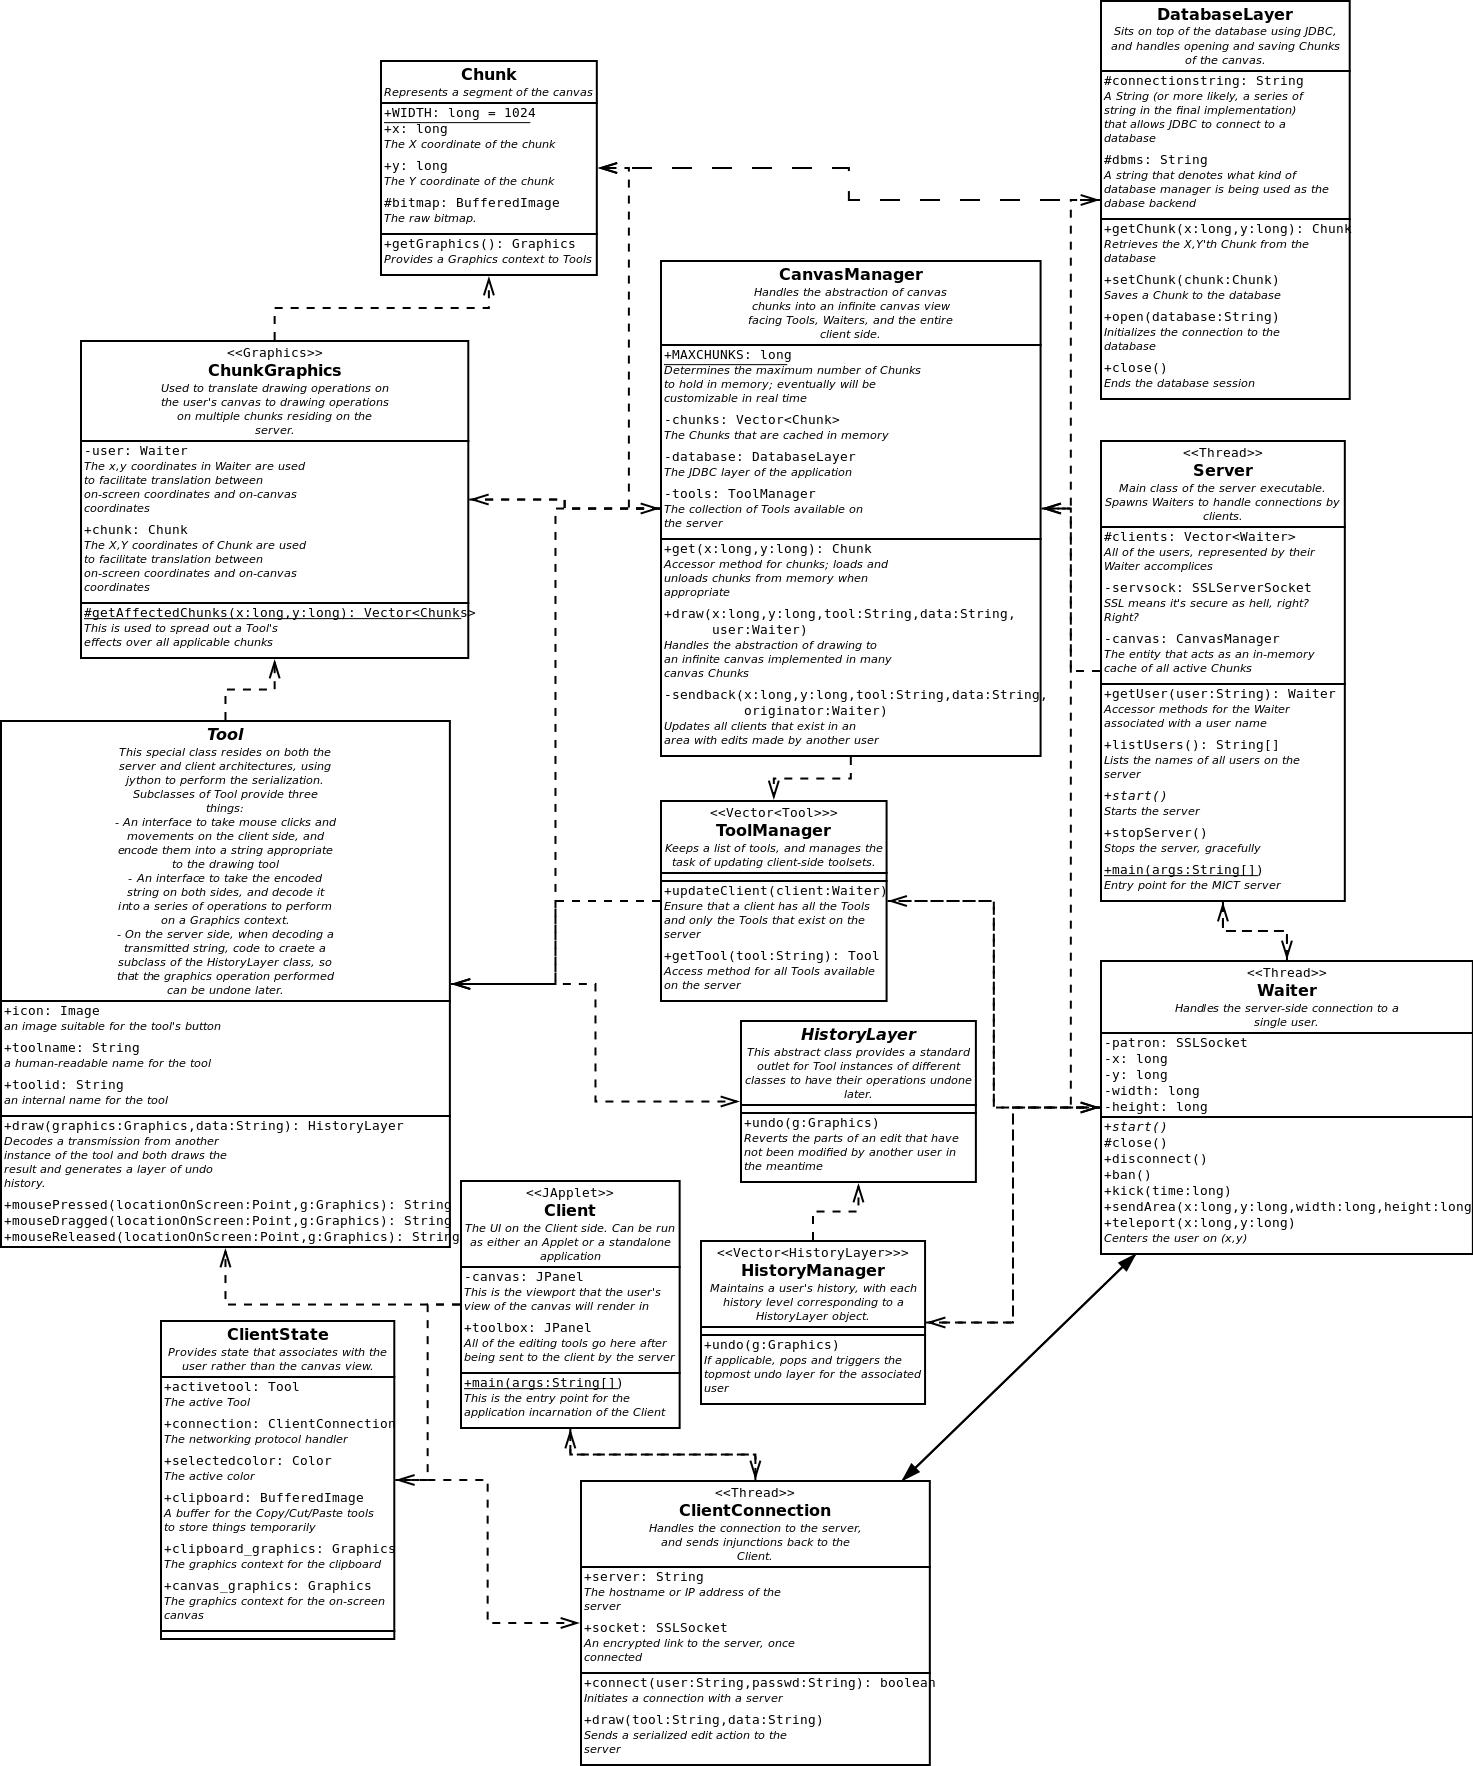
\includegraphics[width=130mm]{design_spec_appendix.png}
 \end{center}
\end{document}
